\documentclass[12pt]{article}

\usepackage{times}
\usepackage{fullpage}
\usepackage{amsfonts,amssymb,amsmath,amsthm}
\usepackage{latexsym}
\usepackage{gauss}
\usepackage{tikz}
\usepackage{tikz-cd}
\usepackage{tkz-graph}
\usepackage{calc}
\usepackage{url}
\usepackage{thmtools}
\usepackage{thm-restate}
\usepackage{hyperref}
\usepackage[capitalise, nameinlink]{cleveref}
\usepackage{algorithm}
\usepackage{algorithmicx}
\usepackage{algpseudocode}
%\usepackage[pdftex]{color}
%\usepackage[breaklinks]{hyperref}
\usepackage{graphicx}
\usepackage{enumitem}
\setcounter{MaxMatrixCols}{15}

%%% Basic notation
\newcommand{\N}{\mathbb{N}}
\newcommand{\Q}{\mathbb{Q}}
\newcommand{\R}{\mathbb{R}}
\newcommand{\Z}{\mathbb{Z}}
\newcommand{\F}{\mathbb{F}}
\newcommand{\E}{\mathbb{E}}
\newcommand{\C}{\mathbb{C}}
\newcommand{\zero}{\mathbf{0}}
\newcommand{\Id}{\mathbf{I}}
\newcommand{\vecu}{\vec{u}}
\newcommand{\Acal}{\mathcal{A}}
\newcommand{\Ccal}{\mathcal{C}}
\newcommand{\Hcal}{\mathcal{H}}
\newcommand{\Lcal}{\mathcal{L}}
\newcommand{\Pcal}{\mathcal{P}}
\newcommand{\Rcal}{\mathcal{R}}
\newcommand{\Kcal}{\mathcal{K}}
\newcommand{\M}{\mathcal{M}}
\newcommand{\Scal}{\mathcal{S}}
\newcommand{\Tcal}{\mathcal{T}}
\newcommand{\Fcal}{\mathcal{F}}
\newcommand{\Gcal}{\mathcal{G}}
\newcommand{\Tr}{\mathrm{Tr}}
\newcommand{\bin}{\mathrm{bin}}
\newcommand{\iu}{\mathrm{i}}
\newcommand{\OR}{\mathrm{i}}
\newcommand{\MAJ}{\mathrm{MAJ}}
\newcommand{\symvec}{\mathrm{symvec}}
\newcommand{\symmat}{\mathrm{Sym}}
\newcommand{\Recover}{\mathsf{RecoverOneFromAll}}
\newcommand{\NULL}{\mathrm{NULL}}
\newcommand{\MINCUT}{\mathrm{MINCUT}}
\newcommand{\CON}{\mathrm{CONNECTIVITY}}
\newcommand{\THRESH}{\mathrm{THRESHOLD}}
\newcommand{\Contract}{\mathrm{Contract}}
\newcommand{\ARGMINCUT}{\mathrm{ARGMINCUT}}
\newcommand{\lin}{\mathrm{lin}}
\newcommand{\cut}{\mathrm{cut}}
\newcommand{\ind}{\mathrm{ind}}
\newcommand{\diag}{\mathrm{diag}}
\newcommand{\IP}{\mathrm{IP}}
\newcommand{\atoms}{\mathrm{atoms}}
\newcommand{\PARITY}{\mathrm{PARITY}}
\newcommand{\upto}{\mathbin{:}}
\DeclareMathOperator*{\argmin}{argmin}
\newcommand{\polylog}{\mathrm{polylog}}
\newcommand{\zeros}{\mathrm{zeros}}
\newcommand{\ones}{\mathrm{ones}}
\newcommand{\rmvec}{\mathrm{vec}}
\newcommand{\rmmat}{\mathrm{mat}}
\newcommand{\laspan}{\mathrm{span}}
\newcommand{\cross}{\mathrm{overlap}}
\newcommand{\coisa}{weighted biadjacency matrix }
\newcommand{\card}[1]{|#1|}
\newcommand{\len}[1]{l(#1)}
\newcommand{\floor}[1]{\lfloor #1 \rfloor}
\newcommand{\ceil}[1]{\left\lceil #1 \right\rceil}
\newcommand{\pair}[2]{\langle #1,#2 \rangle}
\newcommand{\triple}[3]{\langle #1,#2,#3 \rangle}
\def\01{\{0,1\}}

\newcommand{\ith}{i^{\scriptsize \mbox{{\rm th}}}}
\newcommand{\jth}{j^{\scriptsize \mbox{{\rm th}}}}

%\newcommand{\dim}{\mathrm{dim}}
\newcommand{\cd}{\mathrm{cdim}}
\newcommand{\sep}{\mathrm{sep}}
\newcommand{\mer}{\mathrm{mer}}

\DeclareMathOperator*{\argmax}{arg\,max}

\newcommand{\norm}[1]{\|#1\|}


\newcommand{\troy}[1]{\textcolor{red}{#1}}

\newcommand{\bra}[1]{\langle#1|}
\newcommand{\ket}[1]{|#1\rangle}
\newcommand{\bigket}[1]{\big|#1\big\rangle}
\newcommand{\braket}[2]{\langle#1, #2\rangle}
\newcommand{\rk}{\mathrm{rk}}
\newcommand{\I}{\mathcal{I}}
\newcommand{\1}{\mathbf{1}}


\newtheorem{theorem}{Theorem}
\newtheorem{question}[theorem]{Question}
\newtheorem{lemma}[theorem]{Lemma}
\newtheorem{corollary}[theorem]{Corollary}
\newtheorem{proposition}[theorem]{Proposition}
\newtheorem{remark}[theorem]{Remark}
\newtheorem{example}[theorem]{Example}
\newtheorem{claim}[theorem]{Claim}
\newtheorem{fact}[theorem]{Fact}
\newtheorem{hypothesis}[theorem]{Hypothesis}

\theoremstyle{definition}
\newtheorem{exercise}[theorem]{Exercise}
\newtheorem{problem}[theorem]{Problem}
\newtheorem{definition}[theorem]{Definition}

\begin{document}
\title{Problem Set 1}
\date{}
\maketitle

\paragraph*{1. Hadamard}
For $x,y \in \{0,1\}^n$ show that the $(x,y)$ entry of $H^{\otimes n}$ is $\frac{(-1)^{x \cdot y}}{\sqrt{2^n}}$ in two different ways.

\paragraph{2. CNOT}
Construct a CNOT gate from two Hadamards and one controlled $Z$ gate.  

\paragraph*{3. Reading circuits}
\begin{enumerate}
  \item What is the output of the two circuits in \cref{fig:one} and \cref{fig:two}?
  In what way does the circuit in \cref{fig:two} simulate the one with intermediate measurements in \cref{fig:one}?
\begin{figure}
    \centering
    \begin{minipage}{0.45\textwidth}
        \centering
        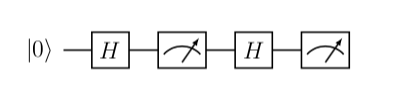
\includegraphics[width=0.9\textwidth]{inter_measure.png} % first figure itself
        \caption{A circuit with intermediate measurements.}
        \label{fig:one}
    \end{minipage}\hfill
    \begin{minipage}{0.45\textwidth}
        \centering
        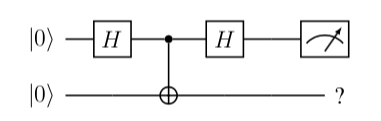
\includegraphics[width=0.9\textwidth]{deferred_measure.png} % second figure itself
        \caption{A circuit with measurement at the end.}
        \label{fig:two}
    \end{minipage}
\end{figure}
  \item Trace the evolution of the states in the circuit in \cref{fig:tele}.  What could this circuit be used for?
\begin{figure}[htb]
\centering
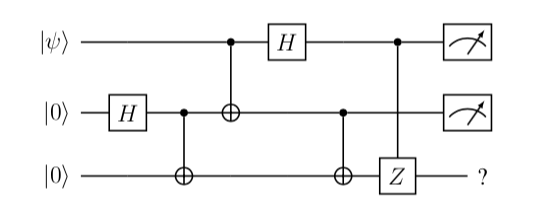
\includegraphics[width=.5\textwidth]{tele_circuit.png}
\caption{$\ket{\psi} = \alpha_0 \ket{0} + \alpha_1 \ket{1}$ is an arbitrary one-qubit state.  What does this circuit do?}
\label{fig:tele}
\end{figure}
\end{enumerate}

\paragraph*{4. Projectors} 
\begin{enumerate}
\item Let $A,B \succeq \mathbf{0}_n$ be $n$-by-$n$ positive semidefinite matrices.  Show that 
\begin{itemize}
  \item $\Tr(AB^*) \ge 0$  
  \item If $\Tr(AB^*) = 0$ then $AB^* = \mathbf{0}_n$.
\end{itemize}
\item Let $P_1, \ldots, P_m \in \C^{n \times n}$ be such that 
\begin{itemize}
  \item $P_i^* = P_i$ and $P_i^2 = P_i$ for all $i =1, \ldots, m$.  That is, each $P_i$ is an orthogonal projector.
  \item $\sum_{i=1}^m P_i = \Id_n$.
\end{itemize}
Show that this implies $P_i P_j = \zero_n$ for all $i \ne j$.  
\end{enumerate}

\paragraph*{5. Simulating randomized circuits}
In lecture we discussed how a randomized circuit can be simulated by a quantum circuit with Hadamard and Toffoli gates 
that allows measurements during the computation.  A cleaner model for quantum circuits, however, is to defer all measurements to the end.  
This exercise is to show that quantum circuits with measurements deferred to the end can also simulate classical randomized circuits.

More precisely, consider a randomized circuit $C$ using Toffoli gates with $n$ input wires, $c$ ancilla wires, $r$ coin toss wires, and $m$ output wires.  
Give a quantum circuit $C'$ using Toffoli, Hadamard, and CNOT gates with $n$ input wires, $c+2r$ ancilla wires, and $m+r$ output wires, such that the probability
distribution over the outcomes on the output wires of $C$ can be simulated by a measurement on $C'$.  Ancillas in $C'$ can be initialized to $\ket{0}$ or $\ket{1}$.  


\paragraph*{6. Only real numbers} 
\begin{enumerate}
  \item Develop a mapping $f: \C \rightarrow \R^{2 \times 2}$ with the properties that for all $z_1, z_2 \in \C$
  \begin{itemize}
    \item $f(z_1) + f(z_2) = f(z_1 + z_2)$.
    \item $f(z_1) \cdot f(z_2) = f(z_1 \cdot z_2)$.
    \item $f(z_1) \cdot f(z_1)^T = |z_1|^2 \Id_2$.
  \end{itemize}
  \item Given a unitary $U \in \C^{n \times n}$ come up with an \emph{orthogonal} matrix $X \in \R^{2n \times 2n}$ such that 
  for any $\ket{z} \in \C^n$ it holds that 
  \[
  X(\ket{0}\ket{\Re(\ket{z})} + \ket{1}\ket{\Im(\ket{z})}) = \ket{0} \ket{\Re(U\ket{z})} + \ket{1}\ket{\Im(U\ket{z})} \enspace .
  \]
  Here $\ket{\Re(\ket{z})} \in \R^n$ is the real part of the vector $\ket{z}$ and $\ket{\Im(\ket{z})} \in \R^n$ is the imaginary part.  (So in 
  general $\ket{\Re(\ket{z})}, \ket{\Im(\ket{z})}$ will be unnormalized states.)
  \item Let $C$ be a quantum circuit on $n$ qubits with 1 and 2 qubit gates.  Design a circuit $C'$ on 
  $n+1$ qubits with real gates on at most 3 qubits such that a measurement in the computational basis on $C$ can be 
  simulated by a measurement on $C'$.
\end{enumerate}

\paragraph*{7. Corrupted Bernstein-Vazirani}
In the Bernstein-Vazirani problem we were given oracle access to the function $f(x) = x \cdot s \bmod{2}$.  
Now suppose that the oracle function is corrupted, that is, it does not always give the correct answer.   Formally, let $e: \{0,1\}^n \rightarrow \{0,1\}$ where $\frac{|e^{-1}(1)|}{2^n} \le \frac{1}{4}$
(here $e^{-1}(1) = \{x: e(x) = 1\}$) and say we have oracle access to the function $f'$ where $f'(x) = x \cdot s + e(x) \bmod{2}$.  Show that there is a quantum query algorithm 
making $1$ query to $f'$ that recovers $s$ with probability at least $\frac{1}{4}$.
\end{document}




















